\svnid{$Id: laufzeitsicht.tex 182 2012-05-24 15:40:41Z dgens001 $}
\chapter{Laufzeitsicht}
\textit{Dieser Abschnitt stellt das Zusammenwirken der Bausteine zur Laufzeit dar.
Es wird dargelegt, wie die zuvor erarbeiteten Anforderungen erfüllt werden, wie die 
Klassen und Bausteine erzeugt, benutzt und beendet werden.}

\section{Charakterbewegung}
Wenn der \gls{Spieler} eine der Steuerungstasten 'W', 'S', 'A' und 'D' für vor- oder rückwärtige bzw.
links- oder rechtsseitige Bewegung (in dieser Reihenfolge) betätigt, wird diese Aktion von 
\textit{TastaturC} per Keyboard-Listener registriert.
Dieser feuert ein Event in Richtung des \gls{Spieler}s, der zuvor beim \textit{TastaturC} als Listener
angemeldet wurde.

Die \textit{Spieler}-Klasse wird aufgefordert ihre \textit{gehe()}-Methode aufzurufen mit der
entsprechenden \textit{Richtung} in Form eines enum-Wertes - den Himmelsrichtungen - als Funktionsparameter.
Bevor die Aktion durchgeführt werden kann, bedarf es einer Überprüfung der Zugänglichkeit des 
betroffenen Nachbarfeldes. 
Bevor die Aktion durchgeführt werden kann, bedarf es einer Überprüfung der Zugänglichkeit des 
betroffenen Nachbarfeldes. \glspl{Feld} implementieren eine \textit{begehbar()}-Methode, die 
Zugänglichkeitsinformationen für jede Richtung in einem Array verwaltet und für die angefragte 
Bewegung einen Wahrheitswert zurückliefert.

\begin{figure}[h]
	\begin{center}
		%trim option's parameter order: left bottom right top , clip = true
		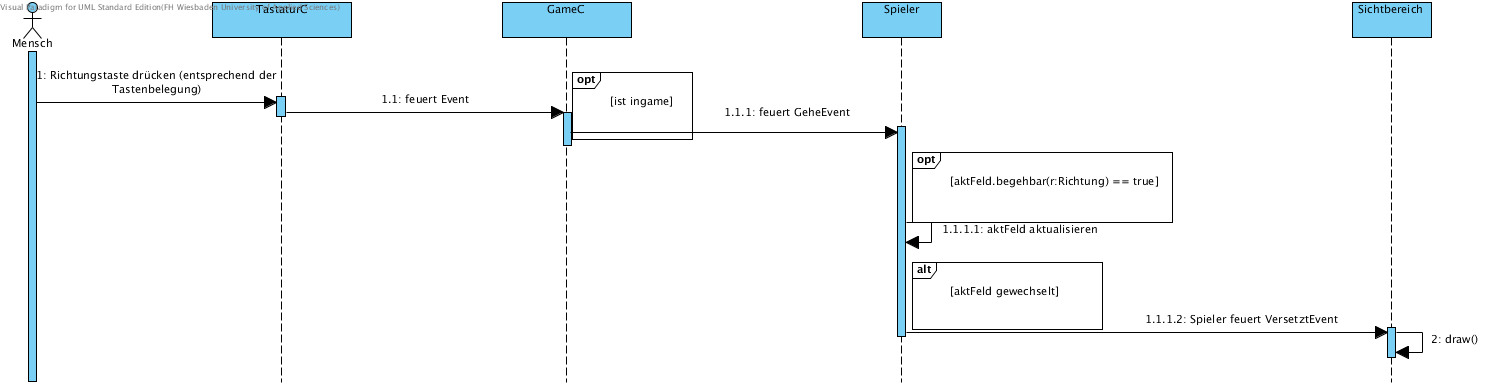
\includegraphics[trim=0cm 0cm 0cm 0cm, clip=true, width=13cm]{kapitel/laufzeitsicht/Spieler_Steuerung.png}
	\end{center}
	\caption{Charakterbewegung}
	\label{fig:steuerung_uml}
\end{figure}

Ist das \gls{Feld} zugänglich wird der \gls{Spieler} versetzt und der \gls{Sichtbereich} wird unter Verwendung der 
Darstellungsinformationen des neuen \gls{Feld}es aktualisiert.
Ist das \gls{Feld} nicht begehbar, wird eine Exception geworfen und der \gls{Spieler} wird per Textanzeige 
darüber informiert.
Auch die Tasten für das Drehen nach links und rechts - 'Q' bzw. 'E' - feuern Events, die
\textit{Spieler}-Klasse veranlassen, ihre \textit{drehe()}-Methode aufzurufen.  Auch sie erhält die gewünschte \textit{Richtung} 
als Parameter.  Das Drehen verändert die Darstellung der \glspl{Feld}, die vor dem \gls{Spieler} liegen, 
nicht aber die des \gls{Feld}es auf dem er sich aktuell befindet.

\section{Interaktion}
Betritt der \gls{Spieler} ein \gls{Feld} auf dem sich ein \gls{npc}, ein \gls{Eingang} zu einem benachbarten \gls{Raum} oder 
\gls{Gegenstand}s befinden, hat er die Möglichkeit, in letzterem Fall diese aufzunehmen bzw., in den beiden 
ersteren, mit ihnen zu interagieren.

Der \gls{Spieler} verwendet das \textit{interagiere}-Interface um mit \textit{Feld} und \textit{NPC} zu interagieren.
Dies geschieht sobald der 
\textit{TastaturC} die Betätigung der Interaktionstaste registriert. Der \gls{Spieler} bekommt zunächst, 
in textueller Form, eine Auflistung der möglichen Interaktionspartner angezeigt. Aus diesen kann 
nun per Zifferntaste einer ausgewählt werden.

\subsection{mit einem NPC}
Jeder von diesen besitzt selbst eine eigene \textit{interagiere()}, welche festlegt was passiert, 
wenn er als Interaktionspartner gewählt wird. Grundsätzlich hat jeder \textit{NPC} einen \textit{Dialog}.
Der \gls{Dialog} liegt in Form einer Baumstruktur vor, aufgebaut aus \glspl{Dialog} und \glspl{Erwiderung}.

\begin{figure}[h]
	\begin{center}
		%trim option's parameter order: left bottom right top , clip = true
		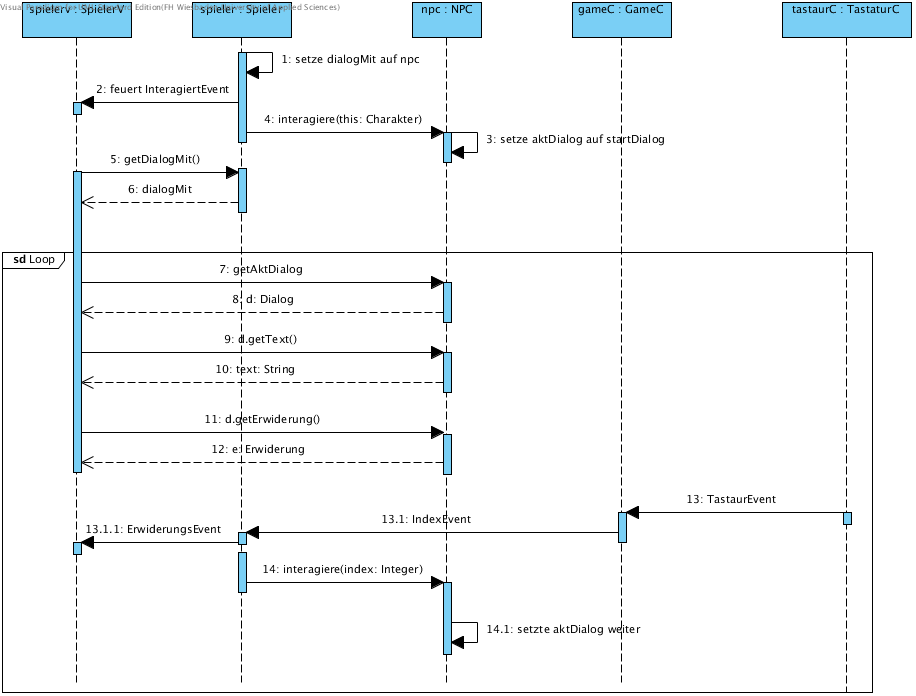
\includegraphics[trim=0cm 0cm 0cm 0cm, clip=true, width=13cm]{kapitel/laufzeitsicht/dialogMitNPC.png}
	\end{center}
	\caption{Dialog mit NPC}
	\label{fig:dialognpc_uml}
\end{figure}

Analog zur Auswahl des Interaktionspartners erfolgt die Wahl der \gls{Erwiderung} über die Zifferntasten.
Manche \gls{npcs} erwarten \glspl{Gegenstand} vom \gls{Spieler}. Im Laufe des \gls{Dialog}es würde an einem festgelegten 
Knoten des Baumes überprüft, ob der entsprechende \gls{Gegenstand} im Handslot des \gls{Spieler}s vorhanden ist.
Ausgehend vom Ergebnis dieser Überprüfung, wird entlang des entsprechenden Astes weiter durch die 
Baumstruktur navigiert.

In der Basisversion der Anwendung ist vorgesehen, dass der \gls{Spieler} die \textit{interagiere()}-Methode des \gls{npcs} 
mit sich selbst als Funktionsparameter aufruft. Hiermit wird ihm signalisiert, dass ein \gls{Dialog} 
gestartet werden soll. Für Erweiterungen sind alternative Interaktionsmöglichkeiten denkbar, 
ausgelöst durch Übergabe weiterer Parameter, wie beispielsweise einer Waffe im Handslot des \gls{Spieler}s.

\newpage

\subsection{mit einem Objekt}
Ein unverschlossener \gls{Eingang}, dessen \textit{interagiere()}-Methode aufgerufen wird, öffnet sich und gibt den 
dahinterliegenden Weg frei.
Ist er aber verschlossen, würde der \gls{Eingang}, ähnlich wie der \gls{npc}, einen \gls{Gegenstand} erwarten. 
Sinnvollerweise eine Art von \textit{Schluessel}, je nach Öffnungsmechanismus. Das matchen von \textit{Schluessel} und 
\textit{Eingang} geschieht anhand ihrer Nummer.

\subsection{mit einem Gegenstand}
In diesem Fall findet keine Interaktion wie in den ersten beiden Fällen statt. Will der \gls{Spieler} einen 
\gls{Gegenstand} vom \textit{Feld} aufnehmen, auf dem er sich aktuell befindet, geschieht das durch das \textit{interagieren}-Interface.

\begin{figure}[h]
	\begin{center}
		%trim option's parameter order: left bottom right top , clip = true
		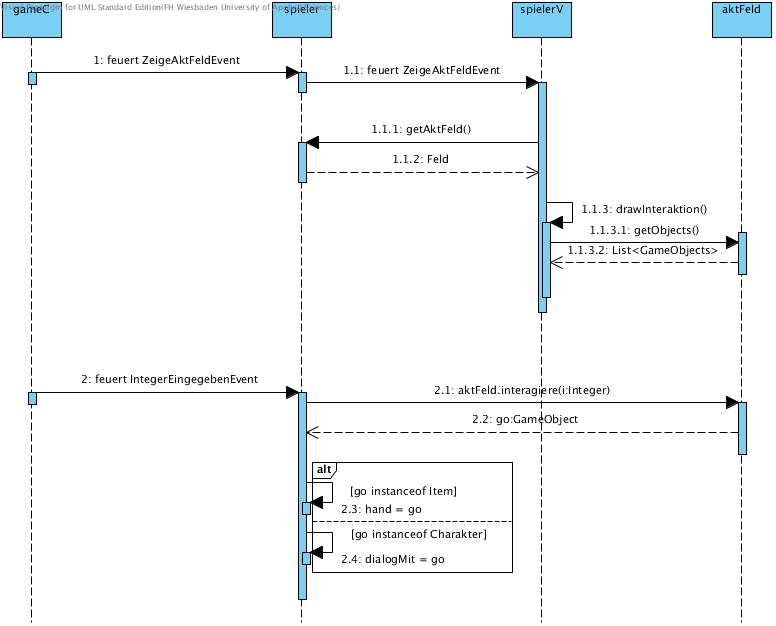
\includegraphics[trim=0cm 0cm 0cm 0cm, clip=true, width=13cm]{kapitel/laufzeitsicht/itemAufnehmen.png}
	\end{center}
	\caption{Gegenstand aufnehmen}
	\label{fig:item_uml}
\end{figure}

Die Referenz im \textit{FeldM} auf das entsprechenden \gls{Gegenstand} wird gelöscht
und eine neue auf den Handslot des \gls{Spieler}s hergestellt. Dieser muss zum Aufnehmen eines neuen \gls{Gegenstand}s 
frei sein. Ist er es nicht, kommt es zur Exception. 
Für spätere Versionen der Anwendung ist es denkbar einen zweiten Handslot einzuführen, der es dann
erlaubt, zwei in den Händen befindliche \glspl{Gegenstand} über ihre \textit{interagiere()}-Methode zu kombinieren.

\subsection{mit dem Inventar}
Möchte der Spieler ein Item aus seinem Handslot in sein Inventar ablegen, geschieht dies ähnlich wie
bei der Übergabe eines Items vom Feld an den Handslot. Die Referenz zwischen Handslot und Item wird 
entfernt, während zwischen Inventar und Item eine neue geschaffen wird.
Soll ein Item aus dem Inventar in den Handslot genommen werden, erhält der Spieler beim Betätigen 
der \textit{inDieHand}-Taste, wieder in textueller Form, eine Auswahl der Gegenstände, die sich in seinem 
Inventar befinden. Per Zifferntaste kann ausgewählt werden. Die Referenzen werden entsprechend 
aufgelöst. Analog zum Feld, stellt das Inventar sowohl eine nehmen-, als auch eine \textit{geben}-Methode 
zur Verfügung.

\begin{figure}[h]
	\begin{center}
		%trim option's parameter order: left bottom right top , clip = true
		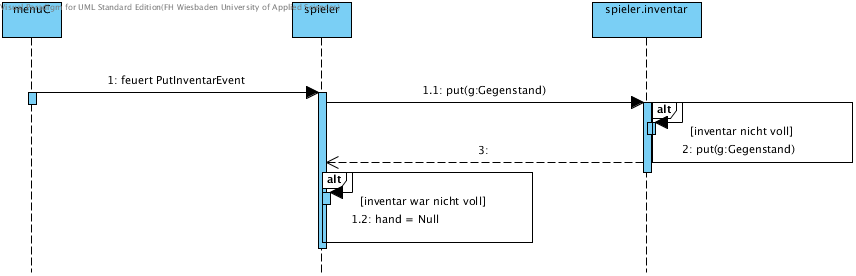
\includegraphics[trim=0cm 0cm 0cm 0cm, clip=true, width=13cm]{kapitel/laufzeitsicht/itemHandInventar.png}
	\end{center}
	\caption{Item ins Inventar}
	\label{fig:inventar_uml}
\end{figure}

\subsection{Neues Spiel}
Der Spieler befindet sich nach dem Spielstart im Hauptmenü. Hier steht ihm die Option Neues Spiel zur 
Verfügung. Startet der Spieler ein neues Spiel ruft dies die \textit{neuesSpiel()}-Methode in \textit{GameC} auf. 
Diese startet die \textit{getGameInstance()}-Methode in der \textit{GameFactory}. Dadurch werden der 
\textit{MapBuilder}, \textit{DialogBuilder} und der \textit{GameObjectBuilder} ausgeführt, welche ein spielbares 
\textit{Ingame} (Spiel) initialisieren. Der \textit{GameC}prüft darauf hin ob ein \textit{Ingame}-Objekt vorhanden 
ist und setzt das Attribut \textit{ingame}(Boolean) entsprechend auf "true". 
Ist der Boolean \textit{ingame} auf true, wird ein Event gefeuert das die \textit{drawIngame()}-Methode der 
\textit{Fenster}-Klasse innerhalb der Darstellungsebene aufruft. Durch \textit{drawIngame()} wird dann die Ansicht 
des Spiels gezeichnet. Zudem startet der \textit{GameC} das Spiel(Gameloop).

\begin{figure}[h]
	\begin{center}
		%trim option's parameter order: left bottom right top , clip = true
		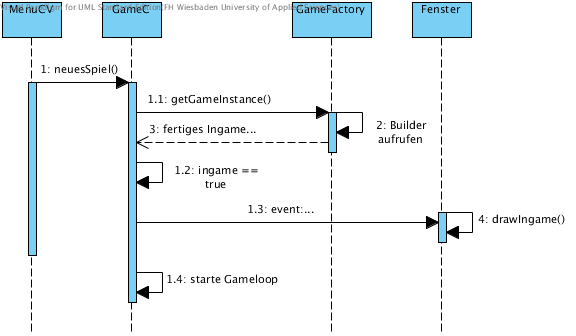
\includegraphics[trim=0cm 0cm 0cm 0cm, clip=true, height=7cm]{kapitel/laufzeitsicht/neuesSpiel.png}
	\end{center}
	\caption{neues Spiel}
	\label{fig:nspiel_uml}
\end{figure}

\newpage

\subsection{Spiel speichern}
Möchte der Spieler seinen aktuellen Spielstand speichern, gelangt er über die entsprechende Taste in das
Pausemenü. Hier findet er den Spiel speichern-Button. Der Spiel speichern-Button löst nach dem betätigen die 
\textit{spielSpeichern()}-Methode des \textit{GameC} aus. Da dieser das Objekt \textit{Ingame} besitzt, kann er die 
\textit{serialisieren()}-Methode der \textit{Ingame}-Klasse aufrufen. Diese speichert alle aktuellen Spieldaten als 
Savegame auf der Festplatte.

\begin{figure}[h]
	\begin{center}
		%trim option's parameter order: left bottom right top , clip = true
		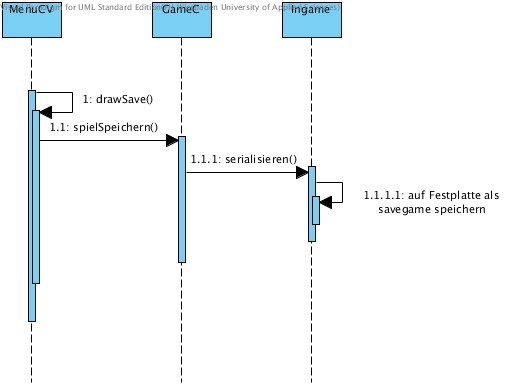
\includegraphics[trim=0cm 0cm 0cm 0cm, clip=true, width=13cm]{kapitel/laufzeitsicht/spiel_speichern.jpg}
	\end{center}
	\caption{Spiel speichern}
	\label{fig:speichern_uml}
\end{figure}
\newpage
\subsection{Spiel laden}
Über das Pausemenü, während einer Spielunterbrechung, oder das Hauptmenü nach dem Spielstart kann der Spieler 
einen Spielstand laden. Wenn ein Spiel geladen werden soll, wird zunächst über die \textit{drawLoad()}-methode des 
\textit{MenuCV} das entsprechende Fenster zur Auswahl eines Savegames gezeichnet. Wurde ein Spielstand gewählt,
wird die \textit{spielLaden()}-Methode zusammen mit dem Savegame als Parameter im \textit{GameC} aufgerufen. 
Der \textit{GameC} startet die \textit{getGameInstanceFromSavegame()}-methode der \textit{GameFactory}, welche das 
übergebene Savegame deserialisiert und ein fertiges \textit{Ingame}-Objekt erstellt. Der \textit{GameC} prüft 
daraufhin ob ein solches spielbares \textit{Ingame}-Objekt vorhanden ist und gibt dann den Boolean \textit{ingame}(true) 
zurück. Ist \textit{ingame} auf true gesetzt feuert der \textit{PropertyChangeListener} ein Event an die 
\textit{Fenster}-Klasse in der Darstellungsebene. Diese zeichnet über die \textit{drawIngame}-Methode das sichtbare Spiel
anhand der des \textit{Ingame}-Objekts, dass aus den Savegamedaten entstanden ist. Zudem startet der \textit{GameC} 
das Spiel.
\\

\begin{figure}[h]
	\begin{center}
		%trim option's parameter order: left bottom right top , clip = true
		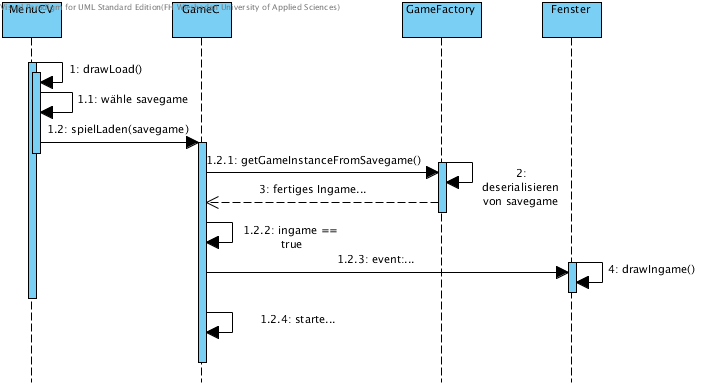
\includegraphics[trim=0cm 0cm 0cm 0cm, clip=true, width=13cm]{kapitel/laufzeitsicht/spielLaden.png}
	\end{center}
	\caption{Spiel laden}
	\label{fig:laden_uml}
\end{figure}
